\subsection{Curve fitting with g2o}

The second practical part of this lecture will introduce another optimized library (mainly in the SLAM field): g2o (General Graphic Optimization, G$^2$O). It is a library based on \textbf{map optimization}. Graph optimization is a theory that combines nonlinear optimization with graph theory, so before we use it, let's take a moment to introduce graph optimization theory.

\subsubsection{Introduction to graph optimization theory}
We have introduced the solution of nonlinear least squares. They are made up of the sum of many error terms. However, there is only one set of optimization variables and many error terms, and we don't know the \textbf{association} between them. For example, how many error terms does an optimization variable $x_j$ exist in? Can we guarantee that the optimization of it makes sense? Further, we hope to be able to visually see the optimization problem \textbf{what it looks like}. Therefore, it involves the optimization of the graph.

Graph optimization is a way to represent optimization problems as \textbf{Graph}. The \textbf{Figure} here is a graph in the sense of graph theory. A graph consists of several \textbf{Vertex}, and the \textbf{Edge} that connects these vertices. Furthermore, \textbf{vertex} is used to represent \textbf{optimized variable}, and \textbf{edge} is used to denote \textbf{error term}. Thus, for any of the above-mentioned forms of nonlinear least squares problem, we can construct a corresponding \textbf{graph}. We can simply call it \textbf{Figure}, or use the definition in the probability map, called \textbf{Bayesian} or \textbf{factor map}.

\autoref{fig:graph-optimization} is a simple example of graph optimization. We use triangles to represent the camera pose nodes, and circles to represent the landmark points, which form the vertices of the graph optimization; at the same time, the solid line represents the motion model of the camera, and the dashed line represents the observation model, which constitute the edge of the graph optimization.  At this point, although the mathematical form of the whole problem is still like \eqref{eq:least-square}, now we can visually see the \textbf{structure} of the problem.  If you want, you can also do \textbf{remove the isolated vertex} or \textbf{the priority of optimizing the number of edges} (or the vertices according to the terminology of the graph theory).  But the most basic graph optimization is to use graph models to express a nonlinear least squares optimization problem. And we can use the certain properties of the graph model to make better optimizations.
	
\begin{figure}[!ht]
	\centering
	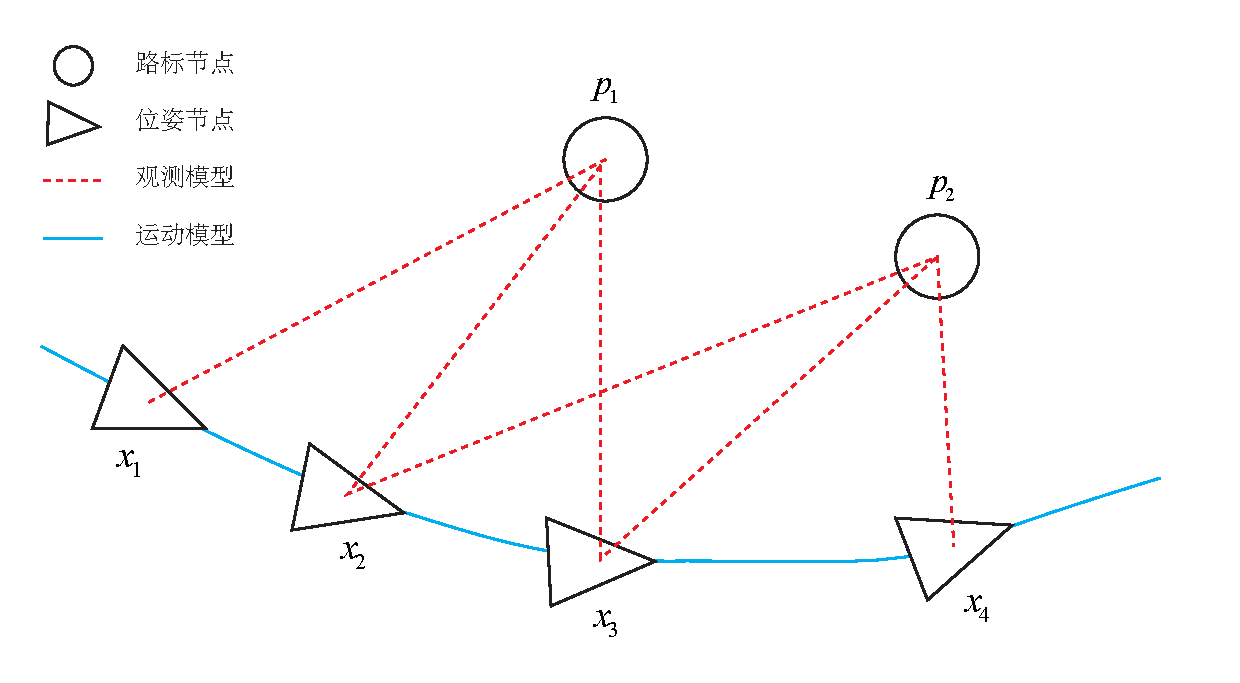
\includegraphics[width=1.0\textwidth]{chapter06/optimization/graphOptimization.pdf}
	\caption{Figure optimization example. }
	\label{fig:graph-optimization}
\end{figure}

G2o is a generic graph optimization library. "Universal" means that you can solve any least squares problem that can be represented as a graph optimization in g2o, obviously including the curve fitting problem discussed above. Let us demonstrate this process.
